\documentclass[11pt, letterpaper]{article}
\usepackage[margin=0.5in]{geometry}
\usepackage{graphicx}

\begin{document}

\title{String Search}
\author{Tavin Turner}
\maketitle

\section{Introduction}
DNA sequences encode the instructions for functions and traits throughout biological organisms. To identify pathways for specific DNA sequences' expression in humans, we must analyze large samples of DNA sequences between individuals. Thanks to the four bases of DNA, we can equivalently solve this problem as computational string search between two strings: the text $T$ and pattern to find instances of $P$. Though there are many approaches to this problem, we analyze the runtime and memory efficiency of naive string search ($O(mn)$ time, $O(1)$ space), which linearly iterates through the text and pattern, and Boyer-Moore, a more sophisticated string search algorithm that avoids shifting to unalignable points ($\Theta(m)$ preprocessing + $O(mn)$ time, $O(m+k)$ space).

\section{Results}
As expected, the runtime of naive string search and Boyer-Moore increased linearly and remained constant in memory with the text size increasing~(Figure \ref{fig:timeandmem}). The space tradeoff in Boyer-Moore's implements are clear, with Naive consistently nearing no space usage, while Boyer-Moore clearly increases with the size of the pattern (the $m$ in $O(m+k)$ space). Since the alphabet is always $\Sigma=\{A,T,G,C\}$, this factor is not observed to change. However, the benefit of Boyer-Moore's higher-memory pre-processing becomes advantageous as early as text only hundreds of characters long. The naive method is roughly equivalent in runtime through the small pattern size changes relative to the text, but Boyer-Moore quickly gained performance with larger and larger pattern sizes, showing that the worst case of Boyer-Moore's runtime is in small pattern sizes, while larger pattern sizes tend closer to its best case $\Omega(n/m)$ matching.

%%%%% Add your experiment here %%%%

\begin{figure}[h!] \centering
    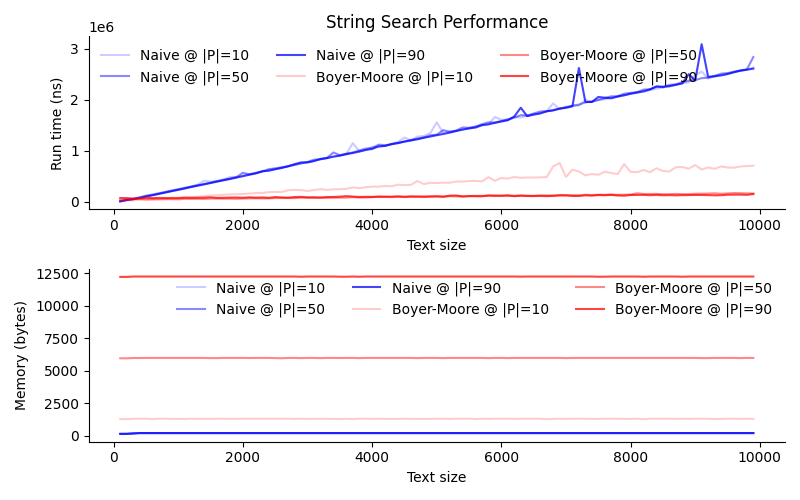
\includegraphics[width=0.6\textwidth]{q100-10000-100_p10-100-40_x5.png}
    \caption{The empirical runtime and memory usage of the naive and Boyer-Moore string search considering a three pattern sizes of 10, 50, and 90 and a database size ranging from 100 to 10,000 characters.}
    \label{fig:timeandmem}
\end{figure}

%%%% Add your figure here %%%%

\section{Methods}

\subsection{Naive string search}
The naive string search algorithm considers all possible alignments of the
pattern $P$ with the text $T$. Staring at the first position in $T$, the
algorithm compares $P$'s characters with the corresponding characters in $T$.
If all characters match, the algorithm records the alignment's position in $T$.
The algorithm then repeats this process for the next alignment. If any of the 
characters in $P$ do not match a corresponding character in $T$, the current
alignment breaks and then $P$ shifts down one position in $T$, and the process
repeats. This process continues until $P$ has been compared to all possible
alignments in $T$, then returns the recorded positions.

\subsection{Boyer-Moore string search}
The Boyer-Moore string search algorithm iteratively considers alignments of the
pattern $P$ with the text $T$, with two key tools to skip clearly non-matching alignments. In preprocessing, the algorithm transforms the string into 1) a bad-character table and 2) a good-suffix table. The bad character table indicates the next-highest-index occurrence of the character at $P[i]$ for all $i$. The good-suffix table gives the highest-index non-suffix occurrence of the sequence matched in $P[i:m]$ with a differing preceding character, or zero otherwise. We then process the text from beginning to end, attempting to align the pattern from its end to beginning on our current offset in the text at each iteration until we match every instance in the string. If we do not match an instance, the pattern is shifted by the maximum potential shift between the bad-character rule and good-suffix rule at that iteration.

\subsection{Empirical comparison}

We evaluated the performance of the naive and Boyers-Moore string search algorithm considering three pattern sizes of 10, 50, and 90 and text sizes that ranged from 100 to 10,000 characters with a step size of 100.  The performance metrics include runtime and memory usage. For each text size, we ran a single search where we generated a random string for $T$ from the alphabet ${A, C, T, G}$ and extracted a random substring $P$ from $T$. We then recorded the runtime and memory usage of the algorithm consider that $P$ and $T$. This was repeated for each text and pattern size five times. After the round was complete for a given text size, we calculated the average runtime and memory usage for the search.

\subsection{Reproducibility}
To replicate these experiments, clone the repository and then run the
following commands from the root directory of the repository.
\begin{verbatim}
$ git clone https://github.com/cu-compg-spring-2025/assignment-4-string-search-itsTurner \
            string_search
$ cd string_search
$ pip install -r requirements.txt
$ python src/string_search.py \
    --text_range 100 10000 100 \
    --pattern_range 10 100 40 \
    --rounds 5 \
    --out_file doc/results/q100-10000-100_p10-100-40_x5.png
\end{verbatim}
%%%% Add your command here%%%%

\end{document}